
\label{sect:photoz}

We evaluate the results of our template training algorithm by using our learned templates to estimate photo-z's for the test set of galaxies using the software package \bpz\ \citep{Benitez2000a}, and comparing the results to the spec-z's and the photo-z's estimated using the original CWW+SB4 templates.
The test set consists of 20,496 galaxies (20\% of the total set), with mean redshift $z_\text{mean} = 0.69$, max redshift $z_\text{max} = 3.61$, and magnitudes $13.8 < i < 25.7$.
See Table \ref{tab:data_sets} for a full summary and Figure \ref{fig:redshift_dist} for the redshift distribution.

\subsection{Bayesian Photometric Redshifts}
\label{sect:bpz}

Bayesian Photometric Redshifts (\bpz; \citealt{Benitez2000a}) is a template-based photo-z estimator.
Template-based estimators take a set of SED templates, assumed to be spanning and exclusive, and calculate observed fluxes over a grid of redshift values.
For each template, \bpz\ evaluates a $\chi^2$ function at each redshift on the grid:
\begin{align}
    \chi^2 (z,T,A) = \sum_n \frac{1}{\sigma_n^2} (\, A \, \hat{f}_n(z,T) - f_n \,)^2,
    \label{eq:chi2}
\end{align}
where $T$ denotes the template, $z$ denotes the redshift, $A$ is a normalization, and $\hat{f}_n$, $f_n$, and $\sigma_n$ denote the calculated flux, the observed flux, and the fractional error as in Equation \ref{eq:cost_function}. 
The sum over $n$ is a sum over the filters for the set of observed fluxes. 
\bpz\ then evaluates the likelihood for producing the observed galaxy fluxes: $p(\{f_n\}|z,T) \propto \exp{(-\chi^2/2)}$. 
The redshift posterior is then calculated by marginalizing over the set of templates:
\begin{align}
    p(z|\{f_n\},m_0) &= \sum_T \, p(z,T|\{f_n\},m_0) \nonumber \\
                     &\propto \sum_T \, p(z,T|m_0) \, p(\{f_n\}|z,T),
\end{align}
where $p(z,T|m_0)$ is a prior over the apparent magnitude $m_0$. 
Work is underway to determine how best to use the full information encoded in the redshift posterior generated by \bpz\ and other photo-z codes (e.g. \citealt{Schmidt2020}). 
In this work, however, only the mode of the posterior distribution is used to estimate the photo-z.

We use \bpz-v1.99.3\footnote{\url{http://www.stsci.edu/~dcoe/BPZ/}} to estimate photo-z's.
We turn off template interpolation by setting \texttt{INTERP=0}.
For simplicity, we treat non-detections as non-observations.
We use the various sets of SED templates described in Section \ref{sect:application}, and use the prior described in the following section.
All other settings were left as default.


\subsection{Galaxy Magnitude Priors}

Before estimating photo-z's with \bpz, we must first construct the magnitude priors, $p(z,T|m_0)$, calibrated to the galaxies in our training set.
We separate the prior into two parts:
\begin{align}
    p(z,T|m_0) = p(T|m_0) \, p(z|T,m_0)
\end{align}
For the magnitude $m_0$, we use one of the $i$ bands in the following order of priority: $i$, $i_2$, $I$, $i^+$.
Instead of constructing a different prior for each template, we follow \citet{Benitez2000a} in dividing our templates into three broad classifications: elliptical (El), spiral (Sp), or irregular/starburst (Im/SB).
The CWW+SB4 templates are already classified under this scheme.
We classify our new templates and each of the galaxies in the training set by assigning the classification of the CWW+SB4 template with the most similar colors, determined by minimizing the mean square error of the fluxes.
The N8 templates are determined to have one elliptical, four spiral, and three irregular/starburst galaxies; the N16 templates are determined to have two elliptical, eight spiral, and six irregular/starburst galaxies.
The fraction of each classification as a function of magnitude for the training set galaxies is displayed in Figure \ref{fig:class_vs_mag}.

We assume that the El and Im/SB galaxies have spectral priors of the form
\begin{align}
    p(T|m_0) = \frac{L_T}{1+e^{-\kappa_T(m_0 - m_T)}} + C_T,
\end{align}
while $p(\text{Sp}|m_0) = 1 - p(\text{El}|m_0) - p(\text{Im/SB}|m_0)$.
The values of $\{L_T,\kappa_T,m_T,C_T\}$ for the El and Im/SB galaxies are found by fitting to the distributions in Figure \ref{fig:class_vs_mag}.
All three priors are plotted in the same figure, and the parameter values are listed in Table \ref{tab:prior_params}.

\begin{figure}
    \centering
    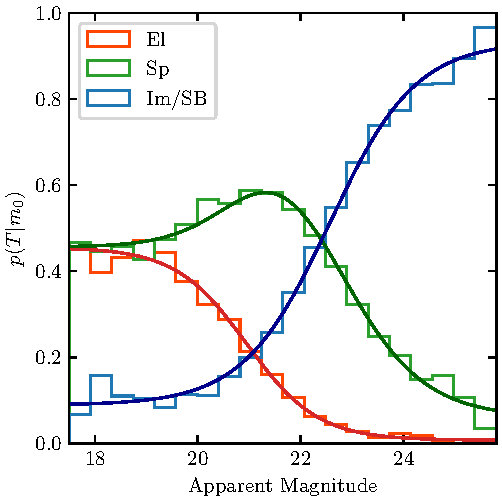
\includegraphics{figures/class_vs_mag.pdf}
    \caption{Fraction of each spectral class as a function of apparent magnitude. The histograms represent the fractions in the training set, and the curves are the spectral type priors fit to the data.}
    \label{fig:class_vs_mag}
\end{figure}

For the redshift prior, we use Equations 23 and 24 from \citet{Benitez2000a}:
\begin{align}
    p(z|T,m_0) = \frac{1}{N_T} \exp \left\{ -\left( \frac{z}{Z_T} \right)^{\alpha_T} \right\},
    \label{eq:z_prior}
\end{align}
where the normalization is
\begin{align}
    N_T = \frac{Z_T^{~\alpha_T + 1}}{\alpha_T} ~ \Gamma \left( \frac{\alpha_T + 1}{\alpha_T} \right),
\end{align}
and the ``median'' redshift $Z_T$ is chosen to have the linear dependence
\begin{align}
    Z_T(m_0) = z_{0T} + k_T(m_0 - 20).
\end{align}
Equation \ref{eq:z_prior} reproduces the exponential cutoff at high redshifts present in the training set, and can reasonably approximate any unimodal redshift distribution, from very narrow ($\alpha \gg 2$) to very broad ($\alpha \ll 1$).
This flexibility reduces the bias introduced by the functional form of the prior \citep{Benitez2000a}.
The nine parameters $\{\alpha_T, z_{0T}, k_T\}$ are determined by maximizing the likelihood $L = \prod_i p(z_i|T_i,m_{0i})$, where the product is over the galaxies in the training set.
The parameters and their bootstrapped uncertainties are listed in Table \ref{tab:prior_params}.

\begin{table*}
    \caption{Parameters for the priors, $p(z,T|m_0)$.}
    \label{tab:prior_params}
    \centering
    \begin{tabular}{l c c c c c c c }
        \hline \hline
         Spectral Type & $L_T$ & $\kappa_T$ & $m_T$ & $C_T$ & $\alpha_T$ & $z_{0T}$ & $k_T$ \\
         \hline
         
         El & $0.448 \pm 0.017$ & $-1.45 \pm 0.16$ & $21.0 \pm 0.1$ & $0.007 \pm 0.009$ & $3.88 \pm 0.04$ & $0.484 \pm 0.003$ & $0.119 \pm 0.002$ \\
         Sp & - & - & - & - & $3.40 \pm 0.04$ & $0.493 \pm 0.003$ & $0.124 \pm 0.002$ \\
         Im/SB & $0.845 \pm 0.031$ & $1.20 \pm 0.11$ & $22.6 \pm 0.1$ & $0.089 \pm 0.013$ & $2.22 \pm 0.03$ & $0.361 \pm 0.009$ & $0.130 \pm 0.008$ \\
        
        \hline
    \end{tabular}
\end{table*}


\subsection{Photo-z Results}
\label{sect:photoz_results}

We estimate photo-z's for the test set galaxies using \bpz\ with the settings and priors described in the previous two sections.
We used four template sets: the original CWW+SB4 templates, the trained CWW+SB4 templates, and the trained N8 and N16 templates.

\bpz\ provides two metrics for the photo-z estimates: \texttt{ODDS} and $\chi_{\text{mod}}^2$.
\texttt{ODDS} measures how narrowly peaked the posterior distribution $p(z|\{f_n\},m_0)$ is around the estimated photo-z.
Galaxies with low \texttt{ODDS} have either broad redshift posteriors, or posteriors with multiple peaks.
$\chi_{\text{mod}}^2$ measures how well the best fit template at the predicted redshift matches the observed fluxes. 
For more about these metrics, see Section 4 of \citet{Benitez2000a} and Section 4.3 of \citet{Coe2006a}.
In this work, photo-z estimates with \texttt{ODDS} $< 0.95$ or $\chi_{\text{mod}}^2 > 1$ are excluded from the analysis, and the fraction excluded on this bases is reported as $f_\text{cut}$.

To further evaluate the results of \bpz, we calculate the scatter, bias, and outlier fraction of the photo-z estimates. 
Photo-z estimates are known to be contaminated with a significant number of outliers.
This is largely driven by a degeneracy wherein the 1000\AA\ Lyman break in a high redshift galaxy spectrum has similar optical colors to the 4000\AA\ Balmer break in a low redshift galaxy spectrum. 
\bpz\ attempts to break this degeneracy with the galaxy magnitude prior (i.e. galaxies with brighter apparent magnitudes are more likely to be at a lower redshift), yet there are still a large number of outliers.

To address this issue, we evaluate the statistics of the interquartile range (IQR) of the data, as these measures are robust to the presence of outliers.
We follow \citet{Graham2018a} in introducing the quantity $\Delta z_{1+z} = (z_{spec} - z_{phot})/(1 + z_{phot})$.
The numerator quantifies the photo-z error and the denominator compensates for the larger uncertainty at high redshifts. 
We define the scatter of the photo-z estimates, $\sigma_\text{IQR}$,  as the width of the IQR in $\Delta z_{1+z}$, divided by 1.349 to convert to the equivalent of a Gaussian standard deviation. 
We define the bias of the photo-z estimates as the mean value of $\Delta z_{1+z}$ for galaxies within the IQR.
The uncertainties of these two values are bootstrapped by calculating the values on 1000 random samples with replacement. 
Outliers are identified as photo-z's with $\Delta z_{1+z} > 3 \sigma_{\text{IQR}}$, and the fraction of outliers is reported as $f_\text{out}$.

\begin{figure*}
    \centering
    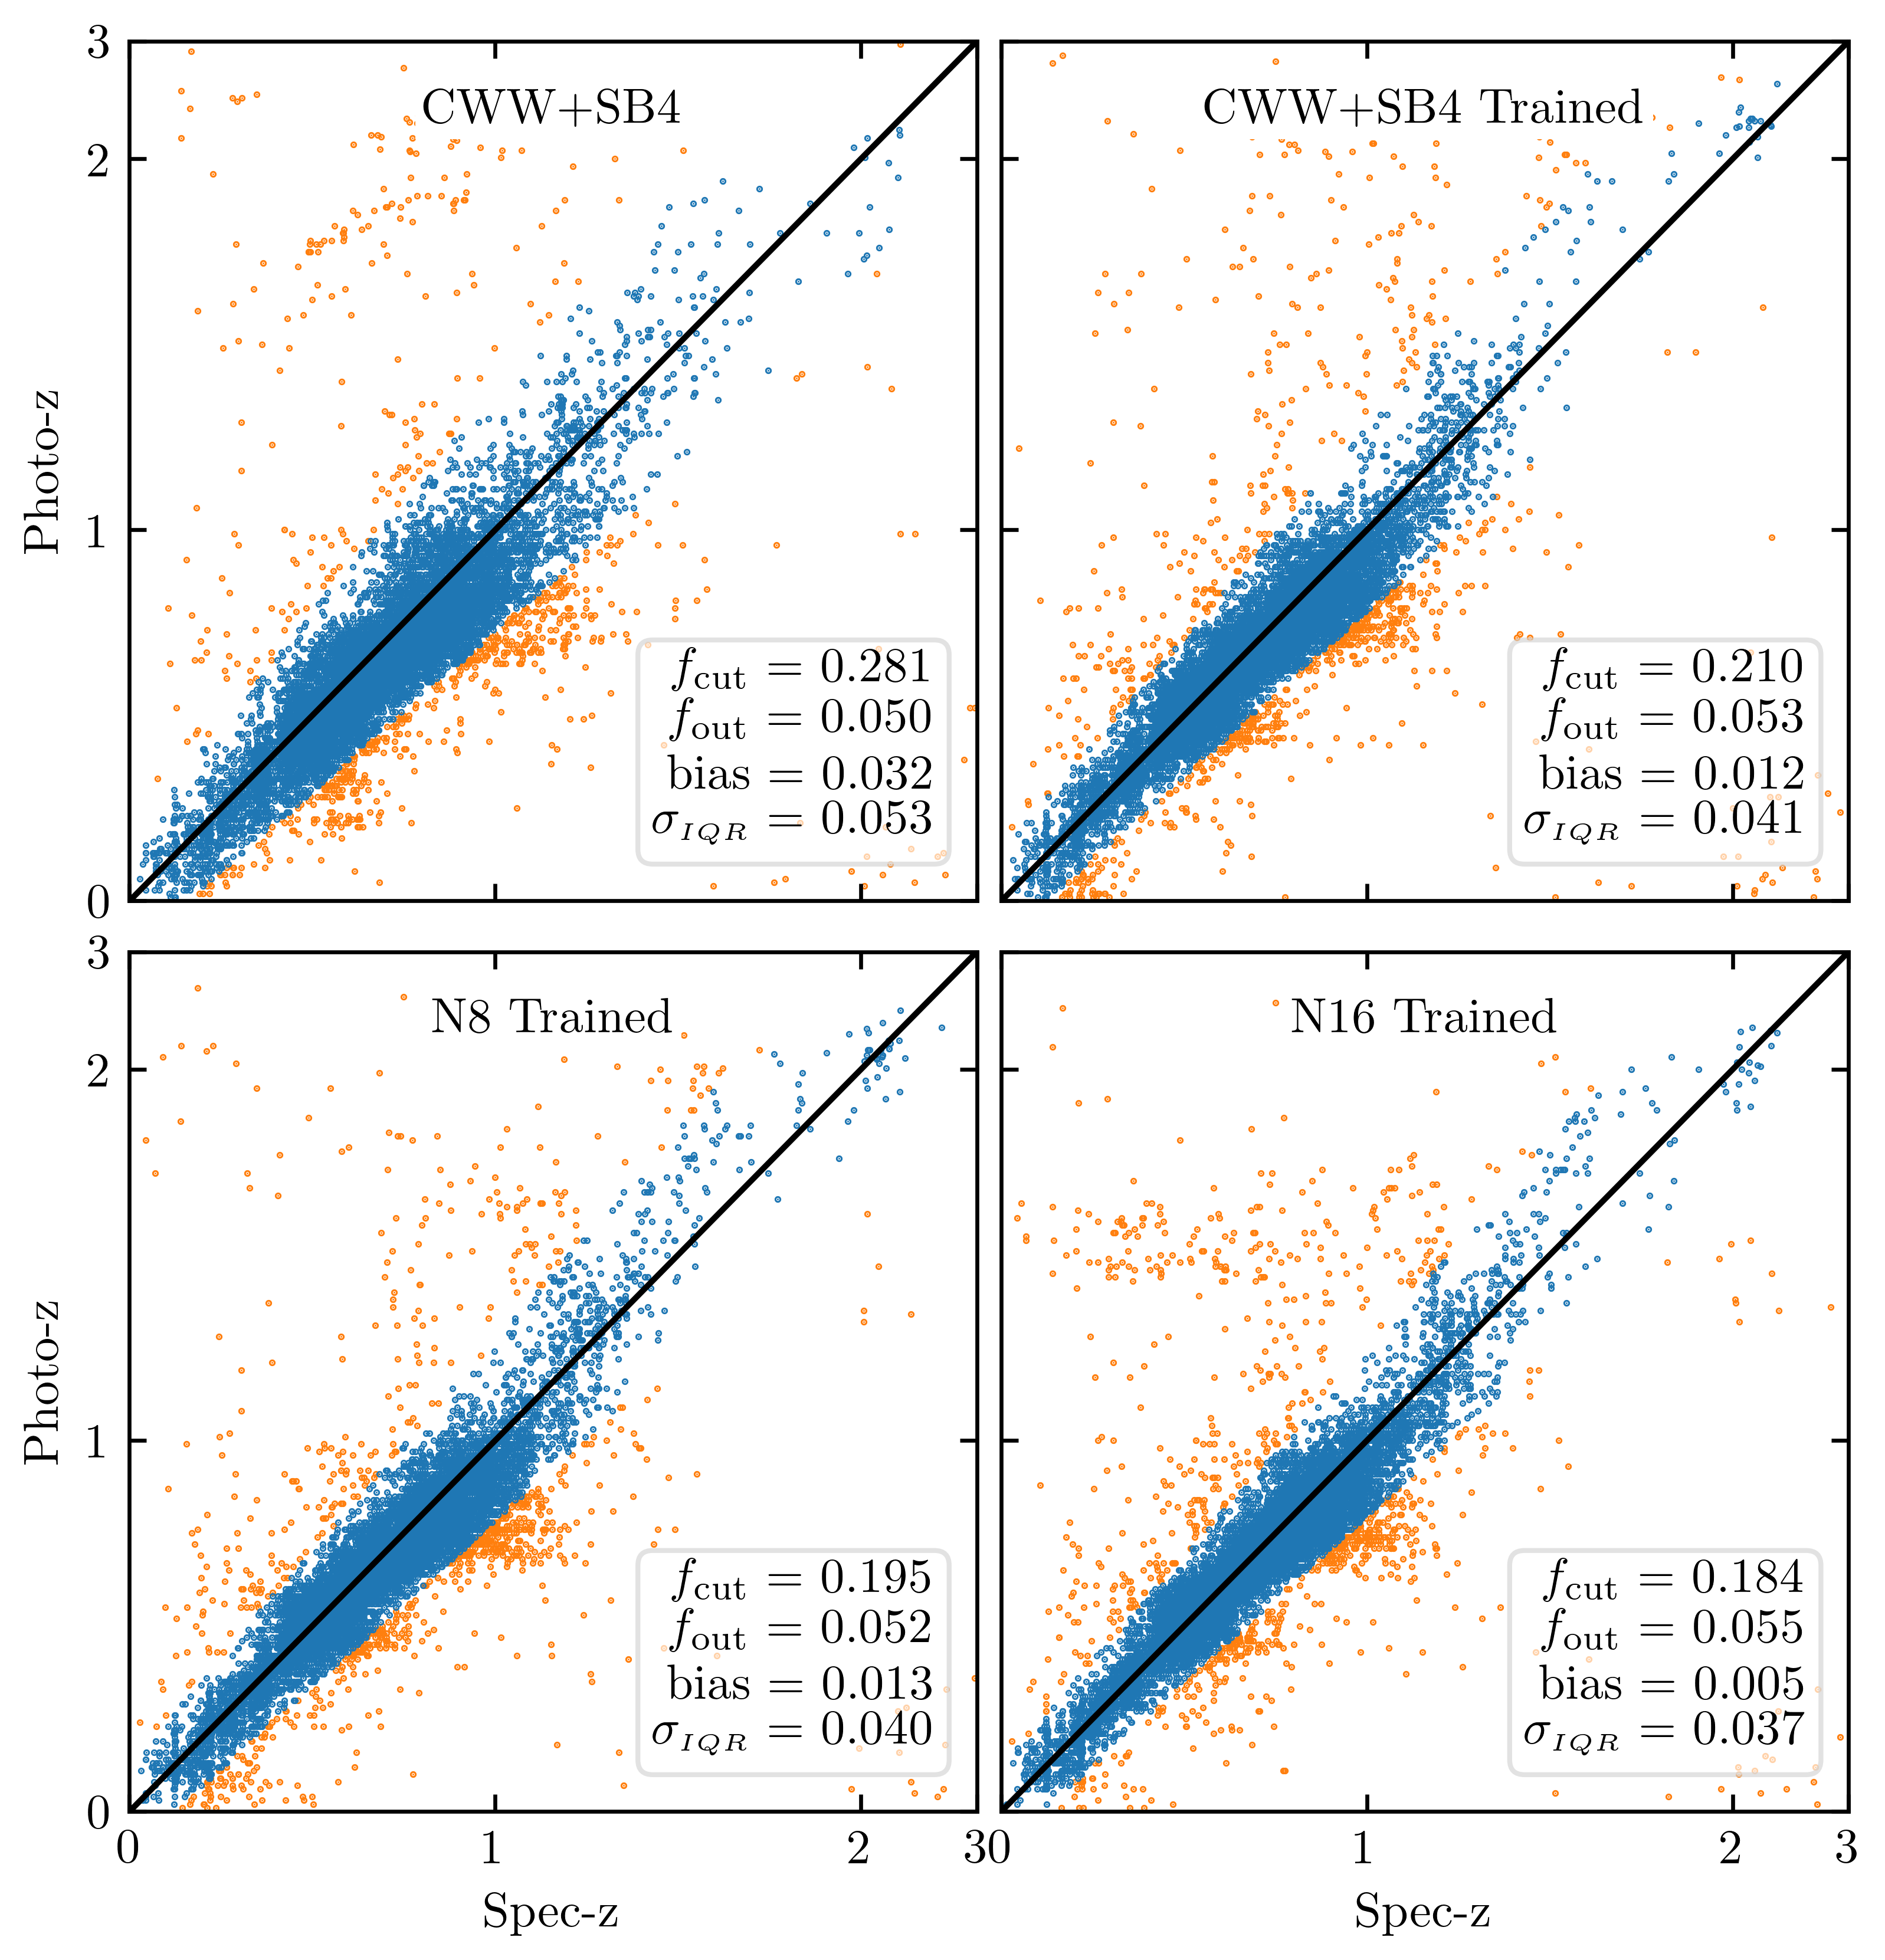
\includegraphics{photoz_results.png}
    \caption{Results of photo-z estimation with \bpz, using the four different templates sets. Photo-z estimates are displayed as points: inliers are blue and outliers are orange. The black line represents perfect estimation (i.e. photo-z = spec-z). The statistics printed in each panel are for the entire data set.}
    \label{fig:photoz_results}
\end{figure*}

The photo-z results can be seen in Figure \ref{fig:photoz_results}.
The photo-z estimates that passed the cuts on \texttt{ODDS} and $\chi_\text{mod}^2$ are displayed as points: the inliers in blue, the outliers in orange.
The values of the photo-z statistics for each template set are printed in each panel.
For all four template sets, the photo-z estimation is reasonably accurate for spec-z's $z < 1.5$.
For higher redshifts, there appears to be a systematic bias towards higher photo-z's.
Reduced photo-z accuracy is generally expected for spec-z's greater than 1.5, as the Balmer break leaves the optical bands at around $z=1.4$ and the Lyman break does not enter the ultraviolet bands until $z=2.5$.

For the CWW+SB4 templates, the training algorithm decreased the fraction of photo-z's cut by 25\%, the bias by 63\%, and the scatter by 23\%, but did not improve the outlier fraction.
We were able to achieve similar photo-z results using the trained N8 and N16 template sets, demonstrating that our training algorithm can be used to generate photo-z templates without any a priori information about galaxy spectra.
Compared to the CWW+SB4 templates, N8 templates decreased $f_\text{cut}$ by 31\%, bias by 59\%, and scatter by 25\%.
The N16 templates decreased $f_\text{cut}$ by 35\%, bias by 84\%, and scatter by 30\%.
In all cases, the training algorithm decreases the fraction of bad photo-z's ($f_\text{cut} + f_\text{out}$), the bias, and the scatter.

Comparing the results for the N8 and N16 template sets indicate that increasing the number of templates can reduce the fraction cut, and the bias and scatter of the photo-z estimates.
To further investigate this relationship, we calculate the photo-z statistics for a range of template numbers, the results of which are in Figure \ref{fig:Ntemplates}.
We find that increasing the number of templates decreases the fraction cut and the bias, as well as slightly decreasing the scatter.
The trend for outlier fraction is less clear.

The N20 set has $f_\text{cut} = 0.188$ (a 33\% decrease compared to CWW+SB4), $f_\text{out} = 0.040$ (a 20\% decrease), bias = 0.003 (a 91\% decrease), and scatter = 0.039 (a 26\% decrease).

\begin{figure*}
    \centering
    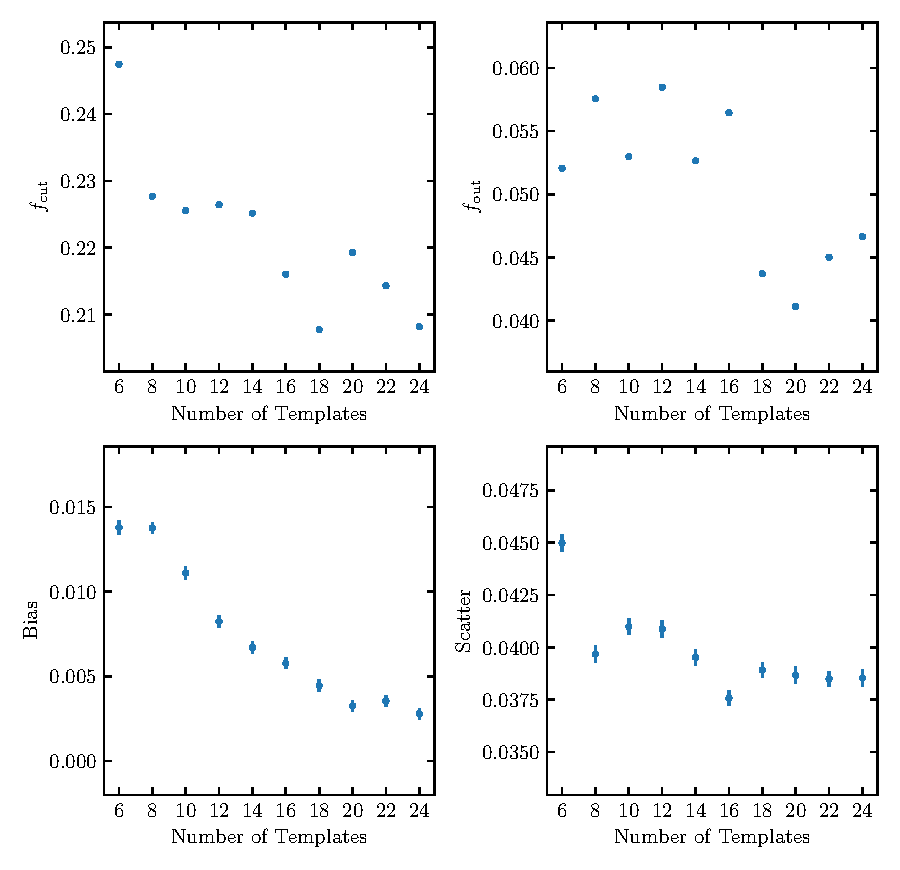
\includegraphics{figures/Ntemplates.pdf}
    \caption{Photo-z statistics as a function of template number. Statistics are for the full redshift range.}
    \label{fig:Ntemplates}
\end{figure*}

The value of the metrics as a function of photo-z can be seen in Figure \ref{fig:photoz_binned}.
In addition to the template sets plotted above, we add the N20 set.
For comparison, plotted in gray are the LSST science requirements for the metrics as listed in the LSST Science Requirement Document (SRD; \citealt{Ivezic2018}).
The SRD lists the following minimum requirements to enable the envisioned LSST cosmological studies: root-mean-square error $< 0.02(1+z_\text{phot})$; $f_\text{out} < 10\%$; average bias $<0.003(1+z_\text{phot})$.
The SRD lists these requirements for an $i<25$, magnitude-limited sample of four billion galaxies from $0.3 < z < 3.0$.
For comparison, our test set consists of 20,496 galaxies with $i < 25.7$, in the range $z < 3.6$, including 19,391 galaxies with $i < 25$, in the range $0.3 < z < 3.0$.
In Figure \ref{fig:photoz_binned}, we show that for redshifts $0.3 < z < 1.2$ we are able to achieve an appropriate outlier fraction, and that our training algorithm makes great progress on the bias, almost reaching the threshold required for LSST.
We also make modest progress on the scatter, but reduction by another factor of two is still required.
Beyond redshift $z=1.2$, all of our metrics far exceed the LSST science requirements.

\begin{figure*}
    \centering
    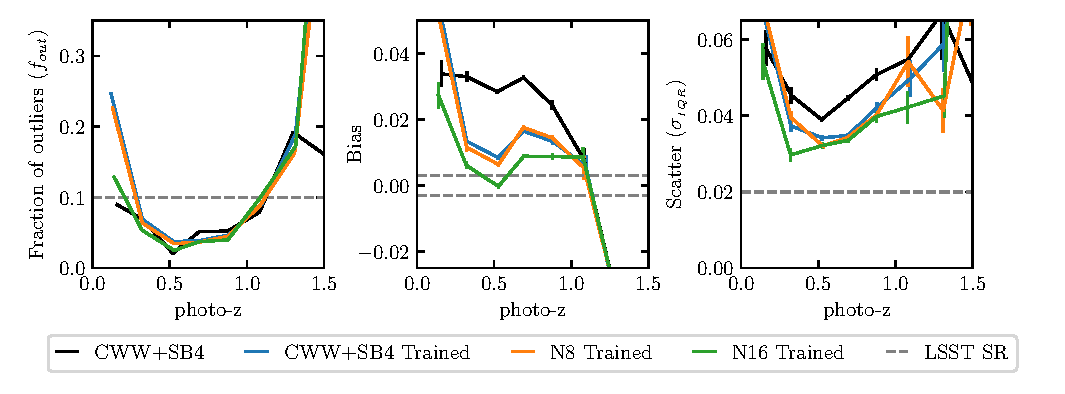
\includegraphics{figures/photoz_binned_metrics.pdf}
    \caption{Photo-z metrics for the various template sets as a function of redshift bin. LSST science requirements are shown as dashed gray lines.}
    \label{fig:photoz_binned}
\end{figure*}